
\documentclass{article}

% Language setting
% Replace `english' with e.g. `spanish' to change the document language
\usepackage[french]{babel}
\usepackage[T1]{fontenc}
\usepackage{listings}

\PassOptionsToPackage{unicode}{hyperref}
\PassOptionsToPackage{naturalnames}{hyperref}
% Set page size and margins
\usepackage[a4paper,top=2cm,bottom=2cm,left=3cm,right=3cm,marginparwidth=1.75cm]{geometry}

% Useful packages
\usepackage{amsmath,amsfonts,amssymb}
\usepackage{graphicx}
\usepackage[colorlinks=true, allcolors=blue]{hyperref}

\title{Introduction : Bases de Haar}
\author{Ina Campan}

\begin{document}
\maketitle

\begin{abstract}

Introduction aux notions de Bases de Haar et de fonctions de Haar.

\end{abstract}

\section{Fonctions de Haar rationnalisées}

On définit une suite de fonctions sur $[0,1]$ par niveaux :

\begin{enumerate}

\item La seule fonction du niveau 0 est la fonction constante égale à $1$.
\item La seule fonction du niveau 1 est égale à $1$ sur [0, 1/2] et égale à $-1$ sur [1/2, 1]
\item Pour $k \geqslant 1$, soit $f$ une fonction du niveau $k$. Alors $f$ est égale à $1$ sur un intervalle $I_1$, égale à $-1$ sur un intervalle $I_2$ et égale à $0$ partout ailleurs. A partir de cette fonction, on définit deux fonctions pour le niveau $k+1$ : la première vaut $1$ sur la première moitié de $I_1$, $-1$ sur la deuxième moitié de $I_1$ et $0$ partout ailleurs; la deuxième fonction vaut $1$ la première moitié de $I_2$, $-1$ sur la deuxième moitié de $I_2$ et $0$ partout ailleurs.

\end{enumerate}

Observation : au $k$-ième niveau, on a $2^{k-1}$ fonctions. La suite de fonctions obtenue s'appelle \textbf{suite des fonctions de Haar}.

\begin{figure}[h]
\centering
\caption{Représentation en python pour le niveau 3.}
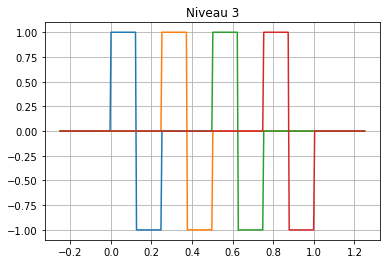
\includegraphics[width=0.5\textwidth]{Images/HaarExempleNiveau3.png}
\end{figure}

%----------------------------------------------------------

\section{Les fonctions de la base de Haar}

On pose : $j \leqslant 0$ et $0 \leqslant k \leqslant 2^j-1$ : 

\[ 
{\psi_{j,k}(x)}= \left\{
\begin{array}{ll}
      2^{\frac{j}{2}} & x \in [k2^{-j}, (k+\frac{1}{2})2^{-j} [\\
      -2^{\frac{j}{2}} & x \in [(k+\frac{1}{2})2^{-j}, (k+1)2^{-j}[ \\
      0 & \text{sinon}
\end{array} 
\right. 
\]

\subsection{Bases Hilbertienne}

Les fonctions de Haar forment une base Hilbertienne de l'espace $\mathbb{L}^2[0,1[$ :

\begin{enumerate}
    \item la suite est orthogonale
    \item la suite est totale : l'espace vectoriel engendré par la suite de fonctions est dense dans $\mathbb{L}^2[0,1[$
\end{enumerate}

\section{Décomposition en base de Haar. Matrices}

\section{Implémentation Python pour les ondelettes}

Il existe une bibliothèque python pour implémenter des codes concernant la compréssion des données :

\begin{lstlisting}

import pywt
from pywt import wavedec
import numpy as np

\end{lstlisting}

\end{document}